\chapter{Materials and Methods}
Self-supervised representation learning is used to obtain visual features from a large scale of unlabeled data. These visual features are discovered by learning the objective function of a pretext task. To assess the quality of features generated by the pretext task, a downstream task based on an application is selected. Knowledge transfer from the pre-trained model in the pretext task proves valuable for the downstream or target task \cite{ericsson_self-supervised_2022}. In this project, the target task is defined as script-type classification for Medieval Latin scripts.

\section{Dataset}

The dataset used in this project comes from the \acrfull{icdar} 2017 competition on the \acrfull{clamm} \cite{cloppet_icdar2017_2017}. All self-supervised models used were pre-trained on a dataset with 70\% of 5,540 images combining the \textit{Training dataset} and \textit{Tasks 1 \& 3 dataset} provided on the competition portal \cite{noauthor_icdar2017-clamm_nodate}. Then, a linear evaluation protocol was followed to evaluate the model's performance and compare it with other models. The subsequent sections detail the setup for the state-of-the-art \gls{ssl} methods used in this project.

\section{Software and Hardware environment}

All the methods were implemented with Pytorch Lightning \cite{Falcon2019} and the Hydra framework \cite{Yadan2019Hydra} for configurations and experiments. The experiments were executed on a High Performance Cluster with \glspl{gpu} using \gls{slurm} jobs. The \glspl{gpu} used for pre-training were Nvidia GeForce RTX3080 and Nvidia A100 Tensor Core.

\section{Self-supervised learning techniques}

\subsection{Simple Framework for Contrastive Learning of Visual Representations}

\gls{simclr} has garnered considerable attention in the machine learning community due to its efficacy in learning meaningful representations from unlabeled data. The \gls{simclr} architecture comprises several key components: a data augmentation module, a base encoder (ResNet-50), a compact projection head, and a contrastive loss function \cite{chen_simple_2020}. In the following discussion, we delve into the configuration of these components.

\begin{itemize}

\item{\textbf{Data augmentation}} module plays a pivotal role and encompasses a sequential series of transformations applied probabilistically. These transformations include random resized crop, horizontal flip, gaussian blur, random rotation, random erasing, dilation, erosion, and normalization. By simulating various nuances found in historical handwritten documents — such as smudging, ink bleeding, discoloration, folds, stains, and others — the augmentations contribute significantly to the model's generalization capabilities.

\item{\textbf{Backbone architecture.}} In order to extract representations from the augmented data, the ResNet-50 neural network encoder architecture is employed. This architecture has been proven effective in capturing relevant features from the input data.

\item{\textbf{Projection head}} serves as a crucial component responsible for reducing the dimensionality of the data. It consists of a sequential neural network comprising two linear layers, with batch normalization and ReLU activation applied in between. This configuration enables the projection head to extract compact representations from the higher-dimensional space.

\item{\textbf{Loss function.}} As recommended by Ting Chen et al. \cite{chen_simple_2020}, the Normalized Temperature-scaled Cross Entropy Loss is employed as the contrastive loss function. This loss function aids in maximizing agreement between differently augmented views of the same sample while minimizing agreement between views of different samples.

\end{itemize}

\begin{figure}[ht]
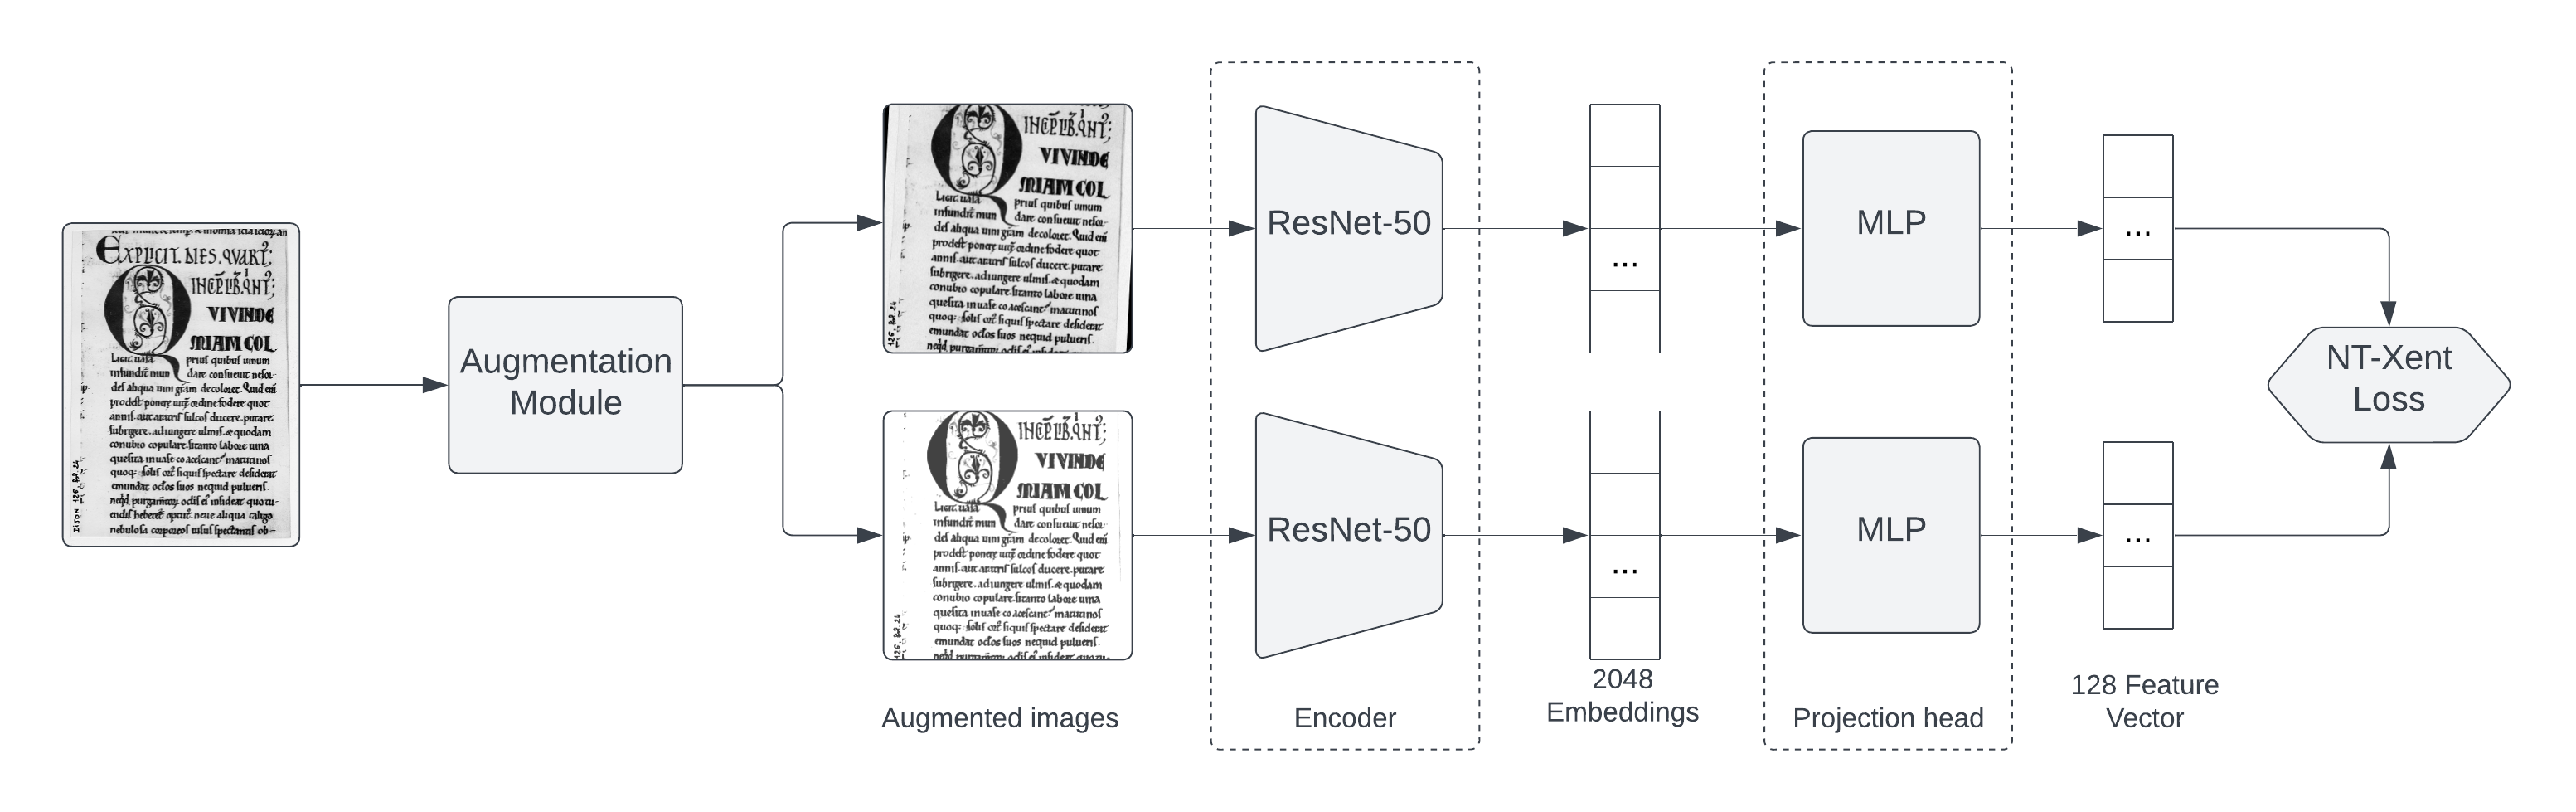
\includegraphics[width=\textwidth]{simclr_arch.png}
\centering
\caption{SimCLR Architecture}
\label{fig:figure}
\end{figure}

\subsection{Masked Autoencoders}
\gls{mae} can serve as powerful pretraining models for deep neural networks. By training an autoencoder on a large unlabelled dataset, it can learn general features or representations that capture the statistical regularities of the data. \gls{mae} comprise two key components: an encoder consisting of \acrfull{vit} blocks in series and a lightweight decoder that reconstructs the input from the representation generated by the encoder. Another essential technique included is an optimal masking ratio of 75\% to balance the accuracy and generalization of the model \cite{he_masked_2021}.

A set of five \gls{vit} architecture sizes from ViT-Tiny to ViT-Huge were evaluated for the encoder. The encoder operates on a visible subset of patches without the mask tokens and a shallow decoder reconstructs the original image from the representation generated by the encoder. Simple transformations of resize, crop and flip are applied. Xavier Uniform technique is used to initialize the weights for all the transformer blocks. The mean squared error at the pixel level between the input and the reconstructed image is used as the loss. 

\begin{figure}[ht]
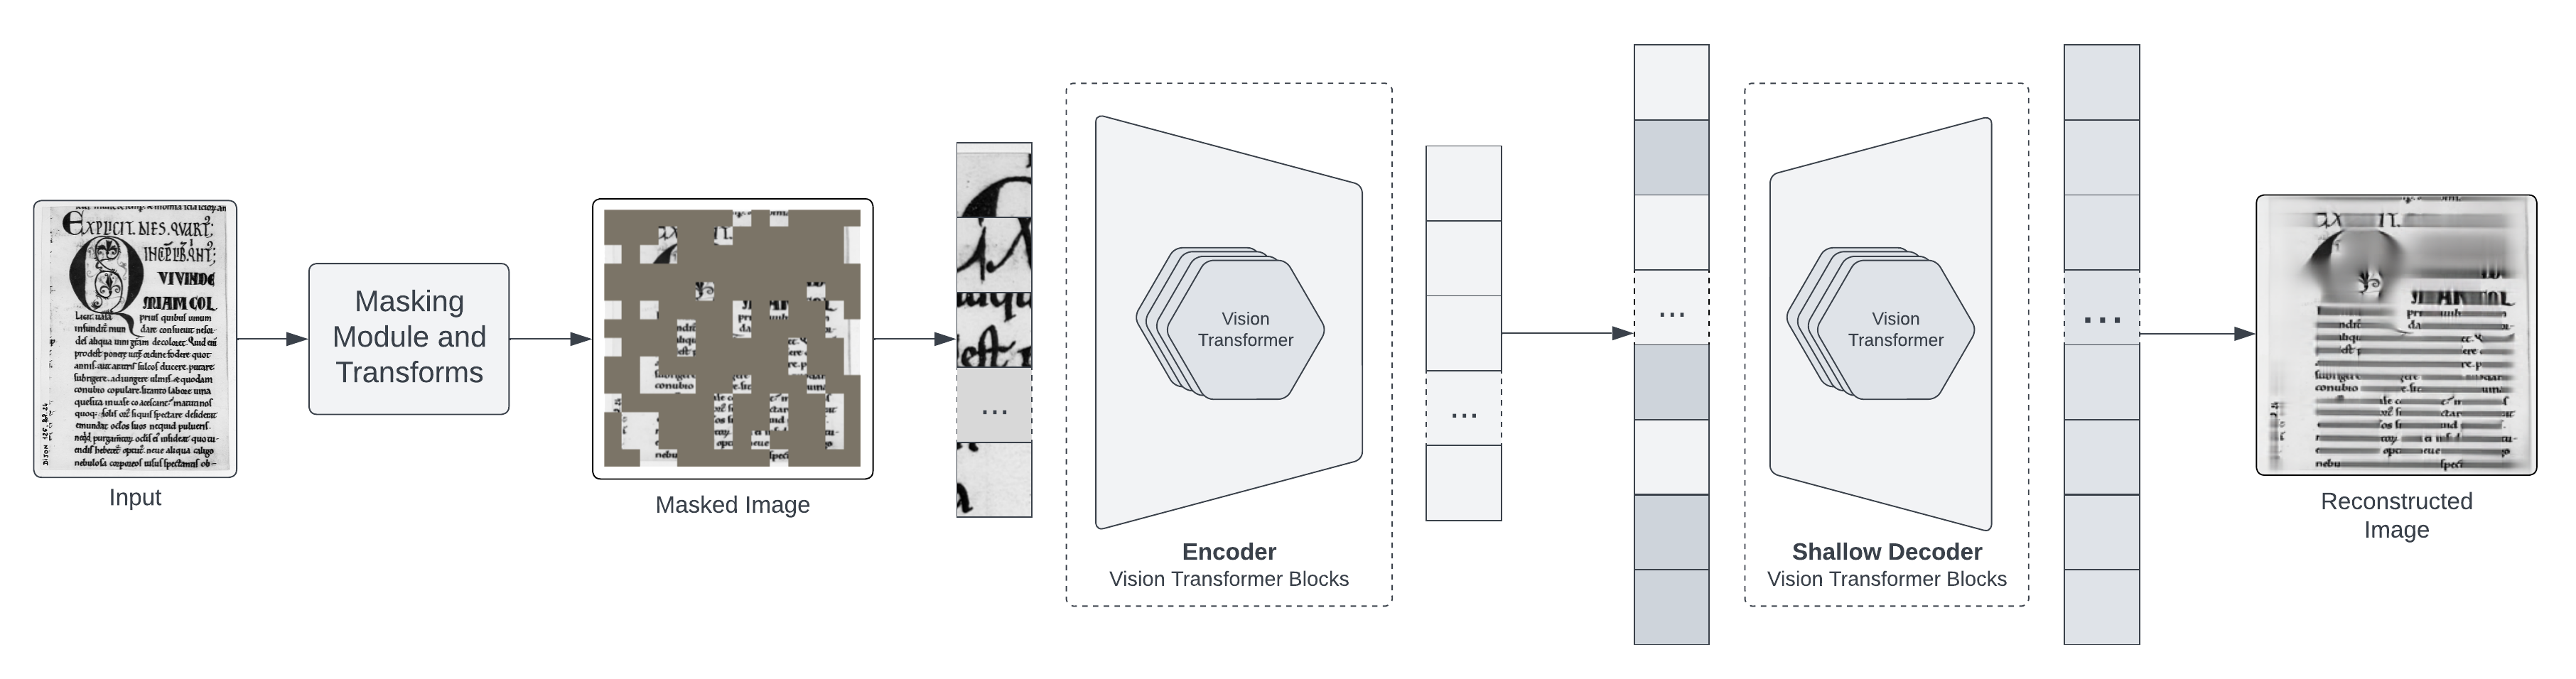
\includegraphics[width=\textwidth]{mae_arch.png}
\centering
\caption{MAE Architecture}
\label{fig:figure}
\end{figure}

\subsection{Bootstrap Your Own Latent}

\gls{byol} uses two neural networks, referred to as the online and target networks, which work together to learn from one another. Both the networks use a ResNet-50 architecture as the backbone and a multi-layer perceptron as the projection network. Additionally, a cosine based similarity loss between the online and target networks plays a vital role in effective learning \cite{grill_bootstrap_2020}. The augmentations for images in the online and target networks are the same as in \gls{simclr}. 

\begin{figure}[ht]
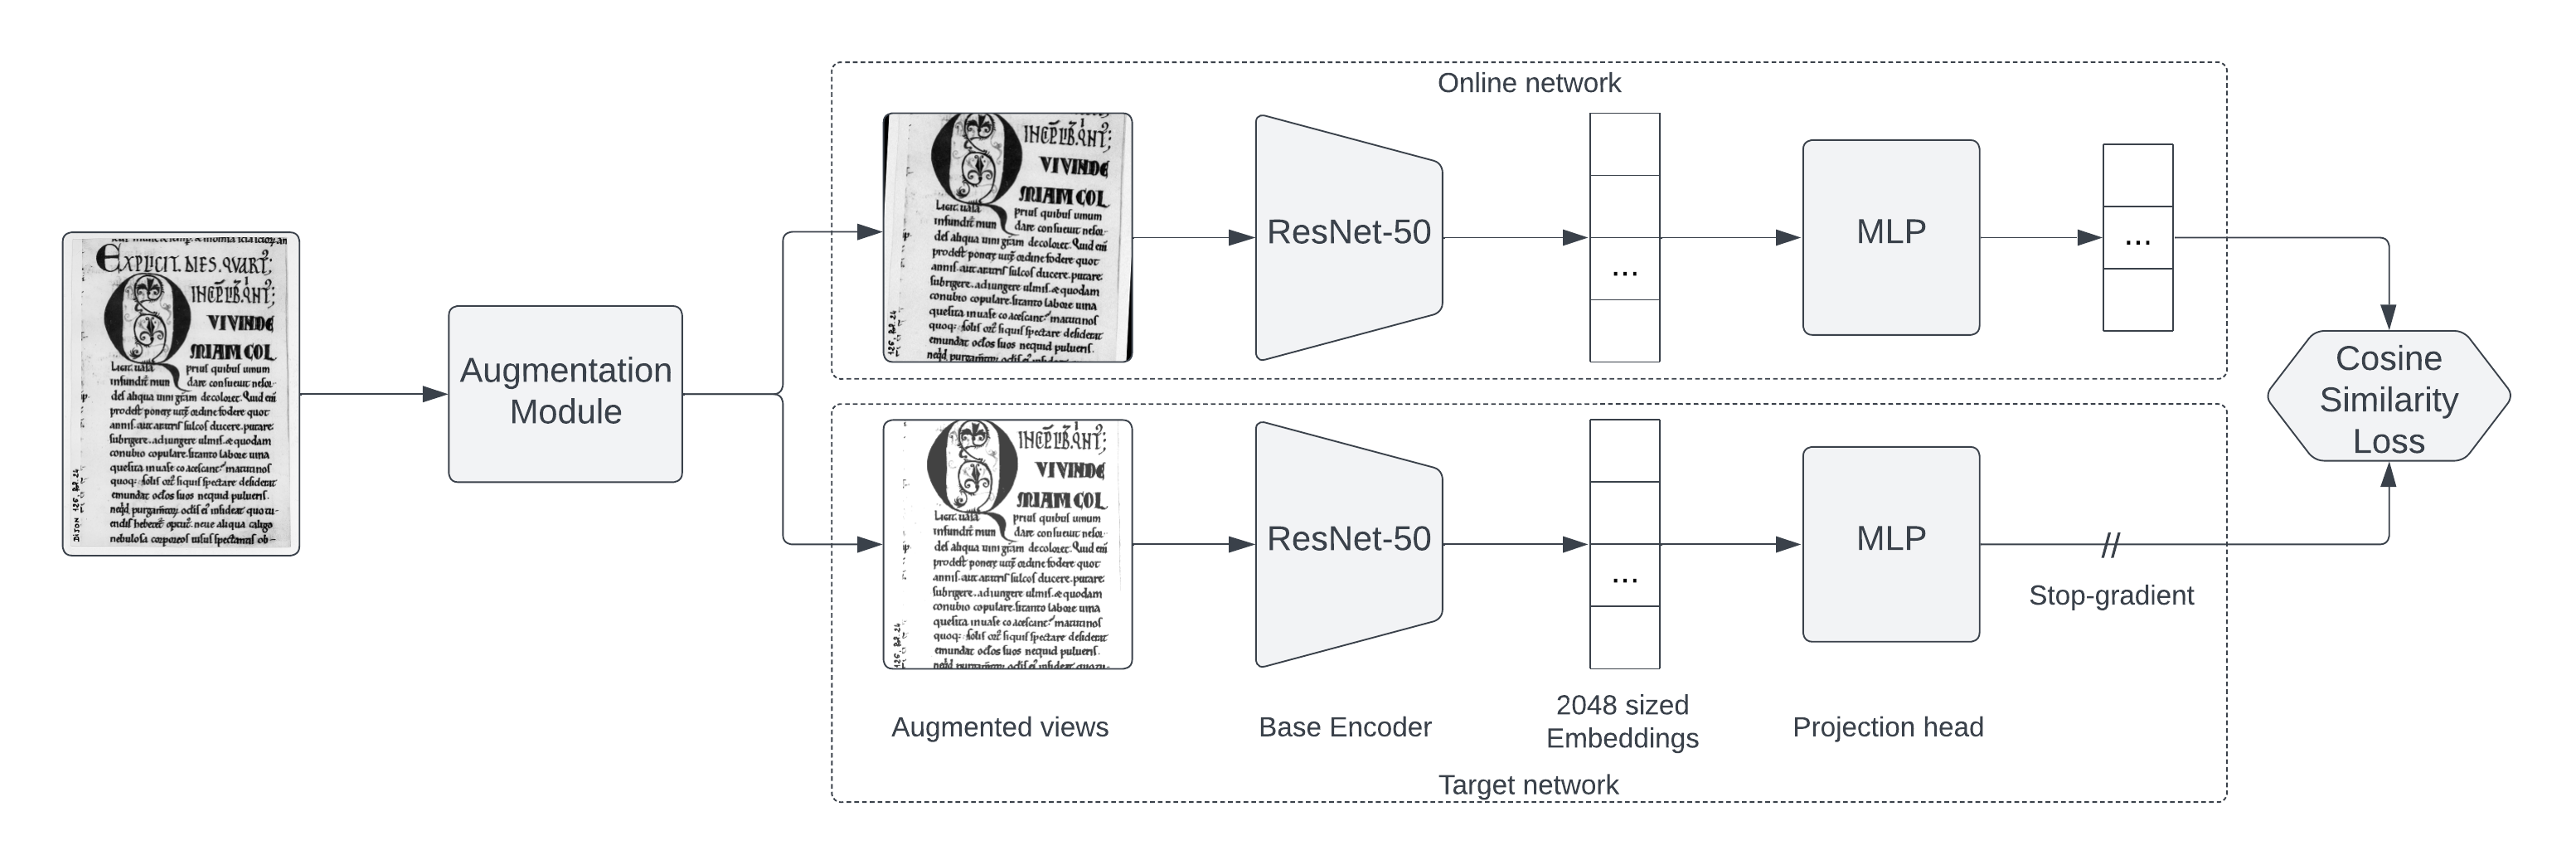
\includegraphics[width=\textwidth]{byol_arch.png}
\centering
\caption{BYOL Architecture}
\label{fig:figure}
\end{figure}
